
\documentclass[10pt,twocolumn,letterpaper,sort&compress]{article}

\usepackage{iccv}
\usepackage{times}
\usepackage{epsfig}
\usepackage{graphicx}
\usepackage{amsmath}
\usepackage{amssymb}
\usepackage[numbers,sort]{natbib}

\usepackage{subfigure}
\usepackage{upgreek}
\usepackage{multirow}
\usepackage{color}
\usepackage{bm}
\DeclareMathOperator*{\argmin}{arg\,min}
\usepackage{arydshln}
\usepackage{latexsym}

\usepackage{amsthm}
\newtheorem{theorem}{Theorem}
\newtheorem{lemma}[theorem]{Lemma}
\newtheorem{conj}[theorem]{Conjecture}


% Include other packages here, before hyperref.

% If you comment hyperref and then uncomment it, you should delete
% egpaper.aux before re-running latex.  (Or just hit 'q' on the first latex
% run, let it finish, and you should be clear).
\usepackage[pagebackref=true,breaklinks=true,letterpaper=true,colorlinks,bookmarks=false]{hyperref}
\renewcommand{\huge}{\fontsize{8pt}{\baselineskip}\selectfont}

% \iccvfinalcopy % *** Uncomment this line for the final submission

\def\iccvPaperID{572} % *** Enter the ICCV Paper ID here
\def\httilde{\mbox{\tt\raisebox{-.5ex}{\symbol{126}}}}

% Pages are numbered in submission mode, and unnumbered in camera-ready
\ificcvfinal\pagestyle{empty}\fi
\begin{document}

%%%%%%%%% TITLE
\title{Multi-channel Weighted Nuclear Norm Minimization for Real Color Image Denoising}

\author{First Author\\
Institution1\\
Institution1 address\\
{\tt\small firstauthor@i1.org}
% For a paper whose authors are all at the same institution,
% omit the following lines up until the closing ``}''.
% Additional authors and addresses can be added with ``\and'',
% just like the second author.
% To save space, use either the email address or home page, not both
\and
Second Author\\
Institution2\\
First line of institution2 address\\
{\tt\small secondauthor@i2.org}
}

\maketitle
%\thispagestyle{empty}

%%%%%%%%% ABSTRACT
\begin{abstract}
The noise structures among the R, G, B channels of real images are quite different due to the preprocessing steps in digital camera pipelines.\ This makes the real image denoising problem much more complex than tranditional grayscale image denoising.\ In this paper, we propose a multi-channel optimization model for real color image denoising.\ Specifically, we introduce a weighting matrix into the data term to process adaptively each part of R, G, B channels in the joint patches concatenated by corresponding patches in these channels.\ In the regularization term, we employ the weighted nuclear norm to exploit the non-local self similar property.\ The proposed multi-channel weighted nuclear norm minimization (MC-WNNM) model is much more complex than the standard WNNM model.\ To solve this new problem, we reformulate the MC-WNNM model into a linear equality-constrained problem and solve it under the alternating direction method of multipliers (ADMM) framework.\ Each alternative updating step has closed-form solution and the convergence results are given.\ Experiments on benchmark datasets demonstrate that the proposed model outperforms state-of-the-art denoising methods on synthetic as well as real-world noisy images.
\end{abstract}

\section{Introduction}

Image denoising is an important problem in enhancing the image quality in computer vision systems. The traditional grayscale image denoising problem aims to recover the clean image $\mathbf{x}$ from the noisy observation $\mathbf{y}=\mathbf{x}+\mathbf{n}$, where $\mathbf{n}$ is often assumed to be additive white Gaussian noise (AWGN). Most image denoising methods in this field either employ the non-local self similarity (NSS) of natural images \cite{nlm,bm3d,ksvd,lssc,ncsr,pgpd,wnnm} or learn generative or discriminative denoisers from paired natural clean images and synthetic noisy images \cite{foe,epll,mlp,csf,chen2015learning}. Among these methods, the weighted nuclear norm minimization (WNNM) method achieves excallent denoising performance by exploiting the NSS property via low rank regularization. 

The real color image denoising problem is not a trivial extension from single channel (grayscale image) to multiple channels (color image). The reason is that the noise in standard RGB (sRGB) space, though could be modeled as AWGN, are with different variances for different channels \cite{Leungtip} due to the on-board processing steps in digital camera pipelines \cite{crosschannel2016,karaimer_brown_ECCV_2016}. This makes the real color image denoising problem much more complex. Directly applying the denoising methods for grayscale images to each channel of color images separately would obtain bad performance \cite{mairal2008sparse}. There are several work  \cite{cbm3d,mairal2008sparse,Liu2008,noiseclinic,crosschannel2016,Zhu_2016_CVPR} proposed specifically for color image denoising. The method \cite{cbm3d} first transforms the color images into the luminance/chrominance space such as YCbCr before denoising, but this would make the noise distribution more complex in color images. The methods of \cite{mairal2008sparse,Zhu_2016_CVPR} process the joint patches concatenated by the corresponding patches in R, G, B channels and treat equally the patches in different channels. This would would generate false colors or artifacts \cite{mairal2008sparse}. The methods of \cite{Liu2008,noiseclinic,crosschannel2016} ignore the non-local self similarity property of natural images, and their performance would be largely depressed \cite{bm3d,wnnm}.

In order to deal with the R, G, B channels in color images more effectively, different noise properties of different channels should be considered in solving real color image denoising problem. Besides, due to its expressive denoising performance, the WNNM model \cite{wnnm} is employed to exploit the NSS property of natural images. In this paper, we proposed a multi-channel WNNM model for real color image denoising. By introducing a weighting matrix to the WNNM model, the proposed multi-channel WNNM model no longer has closed-form solutions and more challenging to solve. By reformulating the proposed multi-channel WNNM model into a linear equality-constrained program with two variables, the relaxed problem can be solved under the alternating direction method of multipliers (ADMM) \cite{admm} framework. Each variable can be updated with closed-form solution \cite{wnnm,lugsvt}. We also give the convergency resutls with detailed proof to guarantee a rational termination of the proposed algorithm. 

\section{Related Work}

\subsection{Weighted Nuclear Norm Minimization}
As an extension to the nuclear norm minimization (NNM) model \cite{cai2010singular}, the weighted nuclear norm minimization (WNNM) model \cite{wnnm} is desribed as 
\vspace{-1mm}
\begin{equation}
\label{e1}
\vspace{-1mm}
\min_{\mathbf{X}}\|\mathbf{Y}-\mathbf{X}\|_{F}^{2}
+
\|\mathbf{X}\|_{\bm{w},*}
\end{equation}
where $\|\mathbf{X}\|_{\bm{w},*}=\sum_{i}w_{i}\sigma_{i}(\mathbf{X})$ is the weighted nuclear norm of matrix $\mathbf{X}$, and $\bm{w}=[w_{1},...,w_{n}]^{\top}, w_{i}\ge 0$ is the weight vector, $\sigma_{i}(\mathbf{X})$ is the $i$-th singular value of matrix $\mathbf{X}$.\ According to the Corollary 1 of \cite{wnnmijcv}, the problem (\ref{e1}) has closed-form solution if the weights are non-decreasing
\vspace{-1mm}  
\begin{equation}
\label{e2}
\vspace{-1mm}
\mathbf{\hat{X}}
=
\mathbf{U}
\mathcal{S}_{\bm{w}/2}
(\mathbf{\Sigma})
\mathbf{V}^{\top}
\end{equation}
where $\mathbf{Y}=\mathbf{U}\mathbf{\Sigma}\mathbf{V}^{\top}$ is the singular value decomposition \cite{eckart1936approximation} of $\mathbf{Y}$ and 
$\mathcal{S}_{\tau}(\bullet)$ is the generalized soft-thresholding operator with weight vector $\bm{w}$:
\vspace{-1mm}
\begin{equation}
\label{e3}
\vspace{-1mm}
\mathcal{S}_{\bm{w}/2}
(\mathbf{\Sigma}_{ii})
=
\max(\mathbf{\Sigma}_{ii}-w_{ii}/2, 0)
\end{equation}

Though having achieved excallent performance on grayscale image denoising, the WNNM model would generate false colors or artifacts \cite{mairal2008sparse}, if being directly extended to real color image denoising by processing each channel separately or joint vectors concatenated by multiple channels. In this paper, for real noisy image denoising, we propose a multi-channel WNNM model which preserve the power of WNNM and be able to process the differences among different channels.

\subsection{Real Color Image Denoising}
During the last decade, several denoising methods are proposed for real color image denoising \cite{cbm3d,Liu2008,Zhu_2016_CVPR,noiseclinic}. Among them, the CBM3D \cite{cbm3d} first transform the RGB image into luminance-chrominance space (e.g., YCbCr) and then apply the famous BM3D method \cite{bm3d} on each channel separately with the patches being grouped only in the luminance channel. In \cite{Liu2008}, the authors proposed the ``Noise Level Function'' to eatimate and remove the noise for each channel in natural images. However, the methods processing each channel separately would achieve inferior performance than processing jointly these channels \cite{mairal2008sparse}. The methods of \cite{noiseclinic,ncwebsite,Zhu_2016_CVPR} perform real color image denoising by concatenating the patches in R, G, B channels into joint vectors. However, the concatenation would treat each channel equally and ignore the different noise properties among these channels. The method in \cite{crosschannel2016} models the cross-channel noise in real noisy image as a multivariate Gaussian and the noise is removed by the Bayesian nonlocal means filter \cite{kervrann2007bayesian}. The commercial software Neat Image \cite{neatimage} estimates the noise parameters from a flat region of the given noisy image and filters the noise correspondingly. But these methods \cite{crosschannel2016,neatimage} ignore the non-local self similarity property of natural images \cite{bm3d,wnnm}. 

In this paper, we introduce a weighting matrix which add differents weights to different channels for color image denoising. The proposed multi-channel method can effectively solve the problem of different noise structures among different channels.

\section{Color Image Denoising via Multi-channel Weighted Nuclear Norm Minimization}

\subsection{The Problem}
\begin{figure*}
\vspace{1mm}
\centering
\subfigure{
\begin{minipage}[t]{0.25\textwidth}
\centering
\raisebox{-0.15cm}{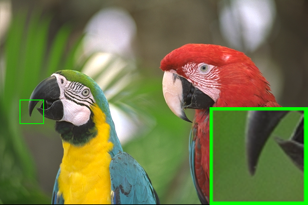
\includegraphics[width=1\textwidth]{example/resize_br_kodim23}}
{\footnotesize (a) kodim23}
\end{minipage}
\begin{minipage}[t]{0.25\textwidth}
\centering
\raisebox{-0.15cm}{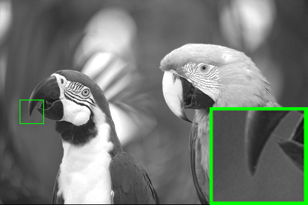
\includegraphics[width=1\textwidth]{example/resize_br_kodim23_1}}
{\footnotesize (b) kodim23: Red Channel}
\end{minipage}
\begin{minipage}[t]{0.25\textwidth}
\centering
\raisebox{-0.15cm}{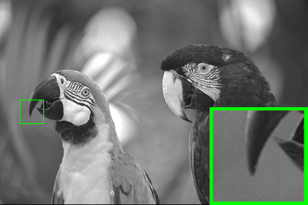
\includegraphics[width=1\textwidth]{example/resize_br_kodim23_2}}
{\footnotesize (c) kodim23: Green Channel}
\end{minipage}
\begin{minipage}[t]{0.25\textwidth}
\centering
\raisebox{-0.15cm}{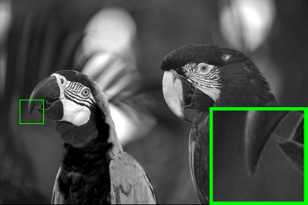
\includegraphics[width=1\textwidth]{example/resize_br_kodim23_3}}
{\footnotesize (d) kodim23: Blue Channel}
\end{minipage}
}\vspace{-4mm}
\subfigure{
\begin{minipage}[t]{0.25\textwidth}
\centering
\raisebox{-0.15cm}{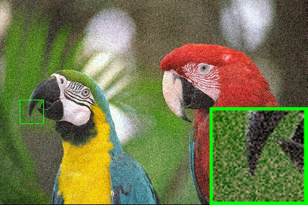
\includegraphics[width=1\textwidth]{example/resize_br_Noisy_nSig402030_kodim23.png}}
{\footnotesize (e) Noisy }
\end{minipage}
\begin{minipage}[t]{0.25\textwidth}
\centering
\raisebox{-0.15cm}{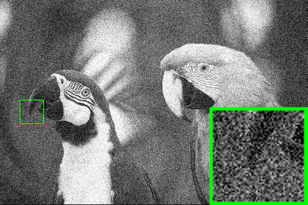
\includegraphics[width=1\textwidth]{example/resize_br_Noisy_nSig402030_kodim23_1.png}}
{\footnotesize (f) Noisy: Red Channel}
\end{minipage}
\begin{minipage}[t]{0.25\textwidth}
\centering
\raisebox{-0.15cm}{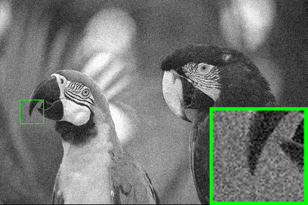
\includegraphics[width=1\textwidth]{example/resize_br_Noisy_nSig402030_kodim23_2.png}}
{\footnotesize (g) Noisy: Green Channel}
\end{minipage}
\begin{minipage}[t]{0.25\textwidth}
\centering
\raisebox{-0.15cm}{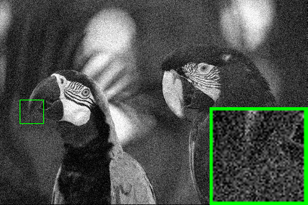
\includegraphics[width=1\textwidth]{example/resize_br_Noisy_nSig402030_kodim23_3.png}}
{\footnotesize (h) Noisy: Blue Channel}
\end{minipage}
}\vspace{-4mm}
\subfigure{
\begin{minipage}[t]{0.25\textwidth}
\centering
\raisebox{-0.15cm}{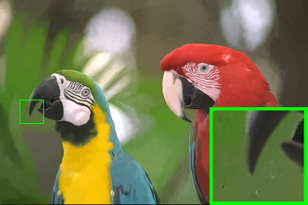
\includegraphics[width=1\textwidth]{example/resize_br_WNNM_nSig402030_lambda1_kodim23.png}}
{\footnotesize (i) WNNM}
\end{minipage}
\begin{minipage}[t]{0.25\textwidth}
\centering
\raisebox{-0.15cm}{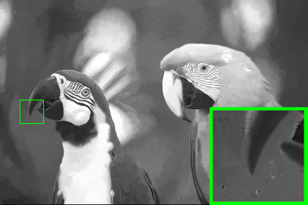
\includegraphics[width=1\textwidth]{example/resize_br_WNNM_nSig402030_lambda1_kodim23_1.png}}
{\footnotesize (j) WNNM: Red Channel}
\end{minipage}
\begin{minipage}[t]{0.25\textwidth}
\centering
\raisebox{-0.15cm}{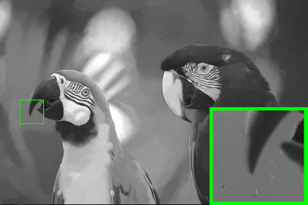
\includegraphics[width=1\textwidth]{example/resize_br_WNNM_nSig402030_lambda1_kodim23_2.png}}
{\footnotesize (k) WNNM: Green Channel}
\end{minipage}
\begin{minipage}[t]{0.25\textwidth}
\centering
\raisebox{-0.15cm}{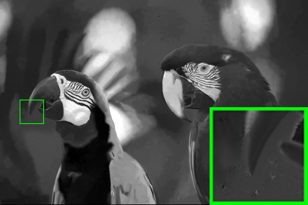
\includegraphics[width=1\textwidth]{example/resize_br_WNNM_nSig402030_lambda1_kodim23_3.png}}
{\footnotesize (l) WNNM: Blue Channel}
\end{minipage}
}\vspace{-1mm}
\caption{The image ``kodim23'' of the Kodak PhotoCD dataset, its degraded version, and the image recovered by WNNM. The R, G, B channels are also listed here for image quality comparison.}
\label{fa}
\vspace{-2mm}
\end{figure*}

The color image denoising problem is to recover the clean image $\{\mathbf{x}_{c}\}$ from its noisy version $\mathbf{y}_{c}=\mathbf{x}_{c}+\mathbf{n}_{c}$, where $c\in \{r, g, b\}$ is the index of R, G, B channels and $\mathbf{n}_{c}$ is the noise in $c$-th channel. The noise structures in each channel are different due to the on-board processing of the digital camera pipelines \cite{karaimer_brown_ECCV_2016}. Therefore, it is problematic to directly apply denoising methods to the joint vectors concatenated by corresponding patches of the R, G, B channels. To validate this point, in Fig.\ \ref{fa}, we show the clean image ``kodim23' taken from the Kodak PhotoCD dataset, its degraded version generated by adding synthetic additive white Gaussian noise (AWGN) to each channel of ``kodim23'', and the denoised image by applying WNNM \cite{wnnm} on the joint vectors concatenated from R, G, B channels of the degraded image. The standard derivations of AWGN added to the R, G, B channels are $\sigma_{r}=40$, $\sigma_{g}=20$, $\sigma_{b}=30$, respectively. The input standard derivation of the noise for the concatenated WNNM method is set as the Root Mean Square (RMS) of those in each channel, i.e., $\sigma=\sqrt{(\sigma_{r}^{2}+\sigma_{g}^{2}+\sigma_{b}^{2})/3}=31.1$. From Fig.\ \ref{fa}, one can see that the concatenated WNNM method treating each channel equally would remain some noise in the R and B channel, while oversmoothing the G channel of the degraded image. Hence, if the patches of different channels are treated adaptively in the concatenated vectors, the degraded color images would be recovered with better visual qualities.

In order to process each channel differently while still exploiting the joint structures of the color images, in this paper, we introduce a weighting matrix $\mathbf{W}$ to the concatenated WNNM method. Assume the matrix $\mathbf{Y}$ containing the noisy patches in R, G, B channels as $\mathbf{Y}=[\mathbf{Y}_{r}^{\top}\ \mathbf{Y}_{g}^{\top}\ \mathbf{Y}_{b}^{\top}]^{\top}$, the corresponding clean matrix $\mathbf{X}=[\mathbf{X}_{r}^{\top}\ \mathbf{X}_{g}^{\top}\ \mathbf{X}_{b}^{\top}]^{\top}$, and the weights $\bm{w}$ for the singular values of $\mathbf{X}$, then the proposed multi-channel WNNM (MC-WNNM) model is
\vspace{-1mm}
\begin{equation}
\label{e4}
\vspace{-1mm}
\min_{\mathbf{X}}\|\mathbf{W}(\mathbf{Y}-\mathbf{X})\|_{F}^{2}
+ 
\|\mathbf{X}\|_{\bm{w},*}.
\end{equation}
How to set the weighting matrix $\mathbf{W}$ and how to solve the proposed model will be introduced in the next sections.



\subsection{The Setting of Weighting Matrix $\mathbf{W}$}
For simplisity, in this paper, we assume the noise are independent among the R, G, B channels and i.i.d. in each channel. Therefore, the weighting matrix $\mathbf{W}$ is diagonal and can be determined under the Bayesian framework:
\vspace{-1mm}
\begin{equation}
\label{e5}
\vspace{-1mm}
\begin{split}
\hat{\mathbf{X}} 
&=
\arg\max_{\mathbf{X}}\ln P(\mathbf{X}|\mathbf{Y},\bm{w})
\\
&
=
\arg\max_{\mathbf{X}}\{\ln P(\mathbf{Y}|\mathbf{X})+\ln P(\mathbf{X}|\bm{w})\}.
\end{split}
\end{equation}
The log-likelihood term $\ln P(\mathbf{Y}|\mathbf{X})$ is characterized by the
statistics of noise, which is assumed to be channel-wise independent white Gaussian with standard deviations $\{\sigma_{r}, \sigma_{g}, \sigma_{b}\}$
\vspace{-1mm}
\begin{equation}
\label{e6}
P(\mathbf{Y}|\mathbf{X}) 
= 
\prod_{c\in\{r, g, b\}}
(2\pi\sigma_{c}^{2})^{-\frac{3p^{2}}{2}}
\exp(-\frac{1}{2\sigma_{c}^{2}}\|\mathbf{Y}_{c}-\mathbf{X}_{c}\|_{F}^{2}).
\end{equation}
We assume that the matrix $\mathbf{X}$ follows the following distribution
\vspace{-1mm}
\begin{equation}
\label{e7}
\vspace{-1mm}
P(\mathbf{X}|\bm{w})
\propto
\exp(-\frac{1}{2}\|\mathbf{X}\|_{\bm{w},*}).
\end{equation}
Putting (\ref{e7}) and (\ref{e6}) into (\ref{e5}), we have
\vspace{-1mm}
\begin{equation}
\vspace{-1mm}
\hat{\mathbf{X}}=\arg\min_{\mathbf{X}}\|\mathbf{W}(\mathbf{Y}-\mathbf{X})\|_{F}^{2}+\|\mathbf{X}\|_{\bm{w},*},
\end{equation}
where
\begin{equation}
\label{e9}
\vspace{-1mm}
\mathbf{W}
=
\left( \begin{array}{ccc}
\sigma_{r}^{-1}\mathbf{I} & \mathbf{0} & \mathbf{0}
\\
\mathbf{0} & \sigma_{g}^{-1}\mathbf{I} & \mathbf{0}
\\
\mathbf{0} & \mathbf{0} & \sigma_{b}^{-1}\mathbf{I}
\end{array} \right).
\end{equation}
where $\mathbf{I}
\in\mathbb{R}^{p^{2}\times p^{2}}$ is the identity matrix. Hence, the weighting matrix $\mathbf{W}$ is determined to contribute equal weights for the pixel values in the same channel, while different weights for those in different channels. The experimental (which will be introduced later) results have already demonstrated that this form of weighting matrix have already generated the best denoising performance on synthetic and real noisy images in  benchmark datasets.




\subsection{The Denoising Algorithm}
In this section, with the proposed MC-WNNM model, we propose a denoising algorithm for color images. In our algorithm, given a noisy image $\mathbf{y}$, each local patch is extracted from it with patch size $p\times p \times 3$ and stretched to a patch vector $\mathbf{y}_{j}\in \mathbb{R}^{3p^{2}}$ concatenated by corresponding patches in R, G, B, channels. Then we search the $M$ most similar patches to $\mathbf{y}_{j}$ (including $\mathbf{y}_{j}$ itself) by Euclidean distance in a $W\times W$ local region around it. We stack the $M$ similar patches column by column to form a noisy patch matrix $\mathbf{Y}_{j}=\mathbf{X}_{j}+\mathbf{N}_{j}\in\mathbb{R}^{3p^{2}\times M}$, where $\mathbf{X}_{j}$ and $\mathbf{N}_{j}$ the corresponding clean and noise patch matrices. Then, we can apply the proposed MC-WNNM model to $\mathbf{Y}_{j}$ to estimate $\mathbf{X}_{j}$ for color image denoising:
\vspace{-1mm}
\begin{equation}
\label{e10}
\vspace{-1mm}
\min_{\mathbf{X}_{j}}
\|
\mathbf{W}_{j}
(\mathbf{Y}_{j}
-
\mathbf{X}_{j})
\|_{F}^{2}
+
\|
\mathbf{X}_{j}\|_{\bm_{w},*}.
\end{equation}
where $\mathbf{W}_{j}$ is defined in Eq.\ (\ref{e9}). Just as \cite{wnnmijcv} did, the weight vector $\bm{w}$ is set $w_{i}^{k+1}=\frac{C}{|\sigma_{i}(\mathbf{X}_{k})|+\epsilon }$ and $\epsilon>0$ is a small number to avoid zero numerator. Note that when $\sigma_{r}=\sigma_{g}=\sigma_{b}$, the multi-channel WNNM model will be reduced to the concatenated WNNM model as a special case.

The multi-channel WNNM is applied to the noisy patch matrix $\mathbf{Y}_{j}$ of each local patch $\mathbf{y}_{j}$ in the noisy image $\mathbf{y}$. And then all the patches are aggregated together to form the final recovered image $\hat{\mathbf{y}}$. To obtain better denoising results, we perform the above denoising procedure for several ($K_{1}$) iterations. The proposed MC-WNNM denoising algorithm for color images is summarized in Algorithm 1.
\begin{table}
\begin{tabular}{l}
\hline
\textbf{Algorithm 1}: Color Image Denoising by MC-WNNM
\\
\hline
\textbf{Input:} Noisy image $\mathbf{y}$, noise levels $\{\sigma_{r}, \sigma_{g}, \sigma_{b}\}$;
\\
\textbf{Initialization:} $\hat{\mathbf{x}}^{(0)}=\mathbf{y}$, $\mathbf{y}^{(0)}=\mathbf{y}$;
\\
\textbf{for} $k = 1:K_{1}$ \textbf{do}
\\
1. Set $\mathbf{y}^{(k)}=\hat{\mathbf{x}}^{(k-1)}$;
\\
2. Extracte local patches $\{\mathbf{y}_{j}\}_{j=1}^{N}$ from $\mathbf{y}^{(k)}$;
\\
\quad\textbf{for} each patch $\mathbf{y}_{j}$ \textbf{do}
\\
3.\quad Search non-local similar patches $\mathbf{Y}_{j}$;
\\
4.\quad Apply the MC-WNNM model (\ref{e10}) to $\mathbf{Y}_{j}$ and
\\
\quad \quad 
obtain the estimated $\mathbf{X}_{j}$;
\\
\quad\textbf{end for}
\\
5. Aggregate $\{\mathbf{X}_{j}\}_{j=1}^{N}$ to form the image $\hat{\mathbf{x}}^{(k)}$;
\\
\textbf{end for}
\\
\textbf{Output:} Denoised image $\hat{\mathbf{x}}^{K_{1}}$.
\\
\hline
\end{tabular}
\vspace{-1mm}
\label{a1}
\end{table}


\subsection{Optimization}
The proposed MC-WNNM model could not be solved in an analytical form while the original WNNM model \cite{wnnmijcv} could. In the WNNM model, when the weights on singular values are non-descending, the weighted nuclear norm proximal operator \cite{wnnmijcv} can have global optimum with closed-form solution. However, such property is not valid for the multi-channel WNNM model. The reason is that the weighting matrix $\mathbf{W}$ is added to the rows of matrix $\mathbf{X}$ instead of its singular values. Besides, the elements in $\mathbf{W}$ is not in a non-descending order with respect to the singular value of $\mathbf{X}$. This makes the proposed model more difficult to solve when compared to the original WNNM model.

By introducing an augmented variable $\mathbf{Z}$, the MC-WNNM model is reformulated as a linear equality-constrained problem with two variables $\mathbf{X}$ and $\mathbf{Z}$:
\vspace{-1mm}
\begin{equation}
\label{e11}
\vspace{-1mm}
\min_{\mathbf{X},\mathbf{Z}}\|\mathbf{W}(\mathbf{Y}-\mathbf{X})\|_{F}^{2}
+
\|\mathbf{Z}\|_{\bm{w},*}
\quad
\text{s.t.}
\quad
\mathbf{X}=\mathbf{Z}.
\end{equation}
Since the objective function is separable across the two variables, the problem (\ref{e11}) can be solved under alternating direction method of multipliers (ADMM) framework. We can derive its augmented Lagrangian function:
\vspace{-1mm}
\begin{equation}
\label{e12}
\vspace{-1mm}
\begin{split}
\mathcal{L}(\mathbf{X},\mathbf{Z},\mathbf{A},\rho)
=
&\|\mathbf{W}(\mathbf{Y}-\mathbf{X})\|_{F}^{2}
+
\|\mathbf{Z}\|_{\bm{w},*}
\\
&
+
\langle
\mathbf{A},\mathbf{X}-\mathbf{Z}
\rangle
+
\frac{\rho}{2}
\|\mathbf{X}-\mathbf{Z}\|_{F}^{2}
\end{split}
\end{equation}
where $\mathbf{A}$ is the augmented Lagrangian multiplier and $\rho>0$ is the penalty parameter. We initialize the matrix variables $\mathbf{X}_{0}$, $\mathbf{Z}_{0}$, and $\mathbf{A}_{0}$ to be zero matrix of suitable size. By taking derivative of the Lagrangian function $\mathcal{L}$ with respect to the variables $\mathbf{X}$ and $\mathbf{Z}$ and setting the derivative function to be zero, we can alternatively update the ADMM algorithm iteratively as follows:
\\
(1) \textbf{Update $\mathbf{X}$ while fixing $\mathbf{Z}$ and $\mathbf{A}$}:
\vspace{-1mm}
\begin{equation}
\label{e13}
\mathbf{X}_{k+1}
=
\arg\min_{\mathbf{X}}
\|\mathbf{W}(\mathbf{Y}-\mathbf{X})\|_{F}^{2} 
+
\frac{\rho_{k}}{2}\|\mathbf{X} - \mathbf{Z}_{k} + \rho_{k}^{-1}\mathbf{A}_{k}||_{F}^{2}
\end{equation}
This is a standard least squares regression problem with closed-form solution:
\vspace{-1mm}
\begin{equation}
\label{e14}
\vspace{-1mm}
\mathbf{X}_{k+1}
=
(\mathbf{W}^{\top}\mathbf{W}+\frac{\rho_{k}}{2}\mathbf{I})^{-1}
(\mathbf{W}^{\top}\mathbf{W}\mathbf{Y} + \frac{\rho_{k}}{2}\mathbf{Z}_{k} -\frac{1}{2}\mathbf{A}_{k})
\end{equation}
\\
(2) \textbf{Update $\mathbf{Z}$ while fixing $\mathbf{X}$ and $\mathbf{A}$}:
\vspace{-1mm}
\begin{equation}
\label{e15}
\mathbf{Z}_{k+1}
=
\arg\min_{\mathbf{Z}}\frac{\rho_{k}}{2}
\|\mathbf{Z} - (\mathbf{X}_{k+1}+\rho_{k}^{-1}\mathbf{A}_{k})\|_{F}^{2}
+
\|\mathbf{Z}\|_{\bm{w},*}
\end{equation}
According to the Theorem 1 in \cite{wnnmijcv}, given the $\mathbf{X}_{k+1}+\rho_{k}^{-1}\mathbf{A}_{k}=\mathbf{U}_{k}\mathbf{\Sigma}_{k}\mathbf{V}_{k}^{\top}$ be the SVD of $\mathbf{X}_{k+1}+\rho_{k}^{-1}\mathbf{A}_{k}$, where 
$\mathbf{\Sigma}_{k}=
\left( \begin{array}{c}
\text{diag}(\sigma_{1},\sigma_{2},...,\sigma_{n})
\\
\mathbf{0}
\end{array} \right)
\in\mathbb{R}^{m\times n}$,
then the global optimum of the above problem is 
$\hat{\mathbf{Z}}=\mathbf{U}_{k}\hat{\mathbf{\Sigma}}_{k}\mathbf{V}_{k}^{\top}$, where 
$\hat{\mathbf{\Sigma}}_{k}=
\left( \begin{array}{c}
\text{diag}(\hat{\sigma}_{1},\hat{\sigma}_{2},...,\hat{\sigma}_{n})
\\
\mathbf{0}
\end{array} \right)
\in\mathbb{R}^{m\times n}$
and $(\hat{\sigma}_{1},\hat{\sigma}_{2},...,\hat{\sigma}_{n})$ is the solution to the following convex optimization problem:
\vspace{-1mm}
\begin{equation}
\label{e16}
\vspace{-1mm}
\begin{split}
\min_{\hat{\sigma}_{1},\hat{\sigma}_{2},...,\hat{\sigma}_{n}}
&
\sum_{i=1}^{n}
(\sigma_{i}-\hat{\sigma}_{i})^{2}
+
\frac{2w_{i}}{\rho_{k}}\hat{\sigma}_{i}
\\
&
\text{s.t.}
\quad
\hat{\sigma}_{1}\ge \hat{\sigma}_{2} \ge...\ge \hat{\sigma}_{n}\ge 0.
\end{split}
\end{equation}
According to the Remark 1 in \cite{wnnmijcv}, the problem above has closed-form solution
\vspace{-1mm}
\begin{equation}
\label{e17}
\vspace{-1mm}
\hat{\sigma}_{i}
=
\left\{ \begin{array}{ll}
0 & \textrm{if $c_{2}<0$}\\
\frac{c_{1}+\sqrt{c_{2}}}{2} & \textrm{if $c_{2}\ge 0$}
\end{array} \right.
\end{equation}
where $c_{1}=\sigma_{i}-\epsilon$, $c_{2} = (\sigma_{i}-\epsilon)^{2}-\frac{8C}{\rho_{k}}$ and $C$ is set as $��
\sqrt{2n}$ by experience in image denoising.
 \\
(3) \textbf{Update $\mathbf{A}$ while fixing $\mathbf{X}$ and $\mathbf{Z}$}:
\vspace{-1mm}
\begin{equation}
\label{e18}
\vspace{-3mm}
\mathbf{A}_{k+1}
=
\mathbf{A}_{k} + \rho_{k}(\mathbf{X}_{k+1}-\mathbf{Z}_{k+1})
\end{equation}
\\
(4) \textbf{Update $\rho_{k}$}: $\rho_{k+1}= \mu * \rho_{k}$, where $\mu>1$.

The above alternative updating steps are repeated until the convergence condition is satisfied or the number of iterations exceeds a preset maximum number, e.g., $K_{2}$. The convergence condition of the ADMM algorithm is: $\|\mathbf{X}_{k+1}-\mathbf{Z}_{k+1}\|_{F}\le \text{Tol}$, $\|\mathbf{X}_{k+1}-\mathbf{X}_{k}\|_{F}\le \text{Tol}$, and $\|\mathbf{Z}_{k+1}-\mathbf{Z}_{k}\|_{F}\le \text{Tol}$ are simutaniously satisfied, where $\text{Tol}>0$ is a small tolerance. We summerize the optimization steps in Algorithm 2. The convergence analysis of the proposed Algorithm 2 is given in Theorem \ref{t1}. Note that since the weighted nuclear norm is non-convex in general, we employ an unbounded sequence of $\{\rho_{k}\}$ here to make sure that the Algorithm 2 is convergent. 

\begin{table}
\begin{tabular}{l}
\hline
\textbf{Algorithm 2}: Solve MC-WNNM via ADMM
\\
\hline
\textbf{Input:} Matrices $\mathbf{Y}$ and $\mathbf{W}$, $\mu>1$, $\text{Tol}>0$;
\\
\textbf{Initialization:} $\mathbf{X}_{0}=\mathbf{Z}_{0}=\mathbf{A}_{0}=\mathbf{0}$, $\rho_{0}>0$, \text{T} = \text{False},
\\
\quad \quad \quad \quad \quad \quad $k=0$; 
\\
\textbf{While} (\text{T} == \text{false}) \textbf{do}
\\
1. Update $\mathbf{X}_{k+1}$ as 
\\
$\mathbf{X}_{k+1}
=
(\mathbf{W}^{\top}\mathbf{W}+\frac{\rho_{k}}{2}\mathbf{I})^{-1}
(\mathbf{W}^{\top}\mathbf{W}\mathbf{Y} + \frac{\rho_{k}}{2}\mathbf{Z}_{k} -\frac{1}{2}\mathbf{A}_{k})
$
\\
2. Update $\mathbf{Z}_{k+1}$ by solving the problem 
\\
\quad 
\quad
$
\min_{\mathbf{Z}}\frac{\rho_{k}}{2}
\|\mathbf{Z} - (\mathbf{X}_{k+1}+\rho_{k}^{-1}\mathbf{A}_{k})\|_{F}^{2}
+
\|\mathbf{Z}\|_{\bm{w},*}
$
\\
3. Update $\mathbf{A}_{k+1}$ as
$
\mathbf{A}_{k+1}
=
\mathbf{A}_{k} + \rho_{k}(\mathbf{X}_{k+1}-\mathbf{Z}_{k+1})
$
\\
4. Update $\rho_{k+1}= \mu * \rho_{k}$;
\\
5. $k \leftarrow k + 1$;
\\
\quad \textbf{if} (Convergence conditions are satisfied) or ($k\ge K_{2}$)
\\
5.\quad \text{T} $\leftarrow$ \text{True}
\\
\quad \textbf{end if}
\\
\textbf{end while}
\\
\textbf{Output:} Matrices $\mathbf{X}$ and $\mathbf{Z}$.
\\
\hline
\end{tabular}
\vspace{-2mm}
\label{a2}
\end{table}

\begin{theorem}
\label{t1}
Assume the weights in $\bm{w}$ are in a non-descending order, the sequence $\{\mathbf{X}_{k}\}$, $\{\mathbf{Z}_{k}\}$, and $\{\mathbf{A}_{k}\}$ generated in Algorithm 1 satisfy:
\begin{align}
&(a) \lim_{k \to \infty} \|\mathbf{X}_{k+1}-\mathbf{Z}_{k+1}\|_{F}=0;
\\
&(b) \lim_{k \to \infty} \|\mathbf{X}_{k+1}-\mathbf{X}_{k}\|_{F}=0;
\\
&(c) \lim_{k \to \infty} \|\mathbf{Z}_{k+1}-\mathbf{Z}_{k}\|_{F}=0.
\end{align}
\end{theorem}
\begin{proof}
We give proof sketch here and detailed proof of this theorem can be found in supplementary files. We can first proof that the sequence $\{\mathbf{A}_{k}\}$ generated by Algorithm \ref{a2} is upper bounded.\ Since $\{\rho_{k}\}$ is unbounded, that is $\lim_{k\to\infty}{\rho_{k}}=+\infty$, we can proof that the sequence of Lagrangian function $\{\mathcal{L}(\mathbf{X}_{k+1},\mathbf{Z}_{k+1},\mathbf{A}_{k},\rho_{k})\}$ is also upper bounded.\
Hence, both $\{\mathbf{W}(\mathbf{Y}-\mathbf{X}_{k})\}$ and $\{\mathbf{Z}_{k}\}$ are upper bounded.\ According to Eq.\ (\ref{e18}), we can proof that 
$
\lim_{k \to \infty} 
\|
\mathbf{X}_{k+1}
-
\mathbf{Z}_{k+1}
\|_{F}
=
\lim_{k \to \infty} 
\rho_{k}^{-1}
\|
\mathbf{A}_{k+1}
-
\mathbf{A}_{k}
\|_{F}
=
0
$,
and (a) is proofed.\ Then we can proof that 
$
\lim_{k \to \infty} 
\|
\mathbf{X}_{k+1}
-
\mathbf{X}_{k}
\|_{F}
\le
\lim_{k \to \infty} 
\|
(\mathbf{W}^{\top}\mathbf{W}
+
\frac{\rho_{k}}{2}
\mathbf{I})^{-1}
(\mathbf{W}^{\top}\mathbf{W}\mathbf{Y}
-
\mathbf{W}^{\top}\mathbf{W}\mathbf{Z}_{k}
-
\frac{1}{2}
\mathbf{A}_{k})
\|_{F}
+
\rho_{k}^{-1}\|
\mathbf{A}_{k}-\mathbf{A}_{k-1}
\|_{F}
=
0
$
and hence (b) is proofed.\ Then (c) can be proofed by checking that 
$
\lim_{k \to \infty} \|\mathbf{Z}_{k+1}-\mathbf{Z}_{k}\|
\le
\lim_{k \to \infty} 
\|
\mathbf{\Sigma}_{k-1}-\mathcal{S}_{\bm{w}/\rho_{k-1}}(\mathbf{\Sigma}_{k-1})
\|_{F}
+
\|
\mathbf{X}_{k+1}-\mathbf{X}_{k}
\|_{F}
+
\rho_{k}^{-1}
\|
\mathbf{A}_{k-1}
+
\mathbf{A}_{k+1}
-
\mathbf{A}_{k}
\|_{F}
=
0
$
,
where $\mathbf{U}_{k-1}\mathbf{\Sigma}_{k-1}\mathbf{V}_{k-1}^{\top}$ is the SVD of the matrix $\mathbf{X}_{k}+\rho_{k-1}\mathbf{A}_{k-1}$
.
\end{proof}

\section{Experiments}
We evaluate the proposed MC-WNNM method on synthetic and real color image denoising. We compare the proposed method with other state-of-the-art denoising methods including CBM3D \cite{cbm3d}, MLP \cite{mlp}, WNNM \cite{wnnm}, TNRD \cite{chen2015learning}, ``Noise Clinic'' (NC) \cite{noiseclinic,ncwebsite}, and the commercial software Neat Image (NI) \cite{neatimage}.

\subsection{Implementation Details}
In synthetic experiments, the noise levels in R, G ,B channels are assumed to be known as $\sigma_{r}, \sigma_{g}, \sigma_{b}$. In the real cases, the noise levels in R, G, B channels can be estimated via noise estimation methods \cite{noiselevel,Chen2015ICCV}. In this paper, we employ the method of \cite{Chen2015ICCV} for its state-of-the-art performance. For the CBM3D method \cite{cbm3d}, the input noise levels are the Root Mean Square (RMS) as 
\vspace{-2mm}
\begin{equation}
\label{e22}
\vspace{-2mm}
\sigma = \sqrt{(\sigma_{r}^{2}+\sigma_{g}^{2}+\sigma_{b}^{2})/3}.
\end{equation}
For the methods of MLP \cite{mlp} and TNRD \cite{chen2015learning}, we retrain the models on grayscale images following their corresponding strategies at different noise levels from $\sigma=5$ to $\sigma=75$ with gap of $5$. The denoising on color images is performed by processing separately each channel with the model trained at the the same (or nearest) noise levels. NC \cite{noiseclinic,ncwebsite} is a blind image denoising method, so we just submit the noisy images (synthetic or real) to \cite{ncwebsite} and perform denoising using the default parameters.\ NI \cite{neatimage} is a commercial software suitable for real image denoising, while the code of CC \cite{crosschannel2016} is not released (but its results on the 15 real noisy images in \cite{crosschannel2016} are available by requesting the authors). Hence, we only compare with CC and NI in real image denoising experiments, and do not compare with them in synthetic experiments. 

In order to take fully comparison with the original WNNM method \cite{wnnmijcv}, we extended the WNNM method \cite{wnnmijcv} for color image denoising in three directions: 1) we apply the WNNM method \cite{wnnmijcv} on each channel separately with corresponding noise levels $\sigma_{r}, \sigma_{g}, \sigma_{b}$. We call this method ``WNNM0''; 2) we perform denoising on the joint vectors concatenated by corresponding patches in the R, G, B channels, where the input noise level $\sigma$ is computed by RMS (Eq.\ (\ref{e22})).\ We call this method ``WNNM1''; 3) we set the weighting matrix $\mathbf{W}$ in the proposed MC-WNNM model as $\mathbf{W}=\sigma^{-1}\mathbf{I}$. For fair comparison, we tune all these methods set the same parameters for ``WNNM2'' and the proposed MC-WNNM methods while achieving the best performance of ``WNNM2''. For fair comparison, we tune the methods of ``WNNM0'', ``WNNM1'', ``WNNM2'', and the proposed MC-WNNM to achieve corresponding best denoising performance (i.e., highest average PSNR results). 

\subsection{Experiments on Synthetic Noisy Images}
In this section, we compare the proposed MC-WNNM method with other competing method \cite{cbm3d,mlp,chen2015learning,noiseclinic,neatimage} as well as the three extensions of WNNM \cite{wnnmijcv} on the 24 high quality color images from the Kodak PhotoCD Dataset (\url{http://r0k.us/graphics/kodak/}), which are shown in Fig.\ \ref{f2}.\ The noisy images are generated by adding additive white Gaussian noise (AWGN) with known standard derivations $\sigma_{r}, \sigma_{g}, \sigma_{b}$ for the R, G, B channels, respectively. In this paper, the noise levels we add to each channel of the 24 color images are $\sigma_{r}=40, \sigma_{g}=20, \sigma_{b}=30$, respectively. More experiments can be found in the supplementary files. For the methods of ``WNNM2'' and MC-WNNM, we set the patch size as $p = 6$, the number of non-local similar patches as $M = 70$, the window size for searching similar patches as $W = 20$, the updating parameter $\mu=1.001$, the number of iterations in Algorithm 1 as $K_{1} = 8$, the number of iterations in Algorithm 2 as $K_{2}=10$. For ``WNNM2'', the initial penalty parameter is set as $\rho_{0}=10$, while for the proposed MC-WNNM model, the penalty parameter is set as $\rho_{0}=3$.

The PSNR results are listed in Table \ref{taba} of the compared methods including CBM3D \cite{cbm3d}, MLP \cite{mlp}, TNRD \cite{chen2015learning}, NI \cite{neatimage}, NC \cite{noiseclinic,ncwebsite}, ``WNNM0'' \cite{wnnmijcv}, ``WNNM1'', ``WNNM2'' and the proposed MC-WNNM methods.\ The best PSNR results are highlighted in bold.\ One can see that on all the 24 images, our method achieves the highest PSNR values over the competing methods.\ On average PSNR, our proposed method achieves 0.48dB improvements over the ``WNNM0'' method and outperforms the ``WNNM2'' by 1.09dB.\ Fig.\ \ref{f3} shows a scene denoised by the compared methods.\ We can see that CBM3D and NC would remain noise while MLP and TNRD would generate artifacts. The methods of ``WNNM0'', ``WNNM1'', ``WNNM2'' would over-smooth much the image.\ By using the proposed MC- WNNM model, our method preserves the structures (e.g., edges and textures) better across the R, G, B channels and generate less artifacts than other denoising methods, leading to visually pleasant outputs.\ More visual comparisons can be found in the supplementary files.

\begin{figure}
\centering
\subfigure{
\begin{minipage}{0.075\textwidth}
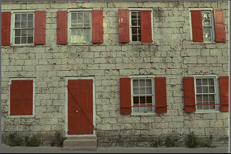
\includegraphics[width=1\textwidth]{24images/resize_kodim01.png}
\end{minipage}
\begin{minipage}{0.075\textwidth}
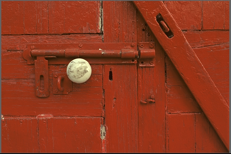
\includegraphics[width=1\textwidth]{24images/resize_kodim02.png}
\end{minipage}
\begin{minipage}{0.075\textwidth}
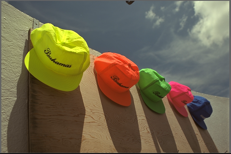
\includegraphics[width=1\textwidth]{24images/resize_kodim03.png}
\end{minipage}
\begin{minipage}{0.075\textwidth}
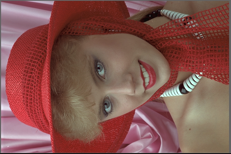
\includegraphics[width=1\textwidth]{24images/resize_kodim04.png}
\end{minipage}
\begin{minipage}{0.075\textwidth}
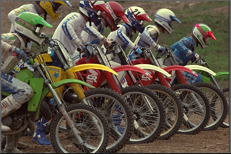
\includegraphics[width=1\textwidth]{24images/resize_kodim05.png}
\end{minipage}
\begin{minipage}{0.075\textwidth}
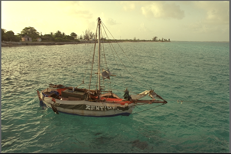
\includegraphics[width=1\textwidth]{24images/resize_kodim06.png}
\end{minipage}
}\vspace{-3mm}
\subfigure{
\begin{minipage}{0.075\textwidth}
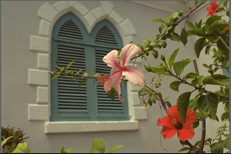
\includegraphics[width=1\textwidth]{24images/resize_kodim07.png}
\end{minipage}
\begin{minipage}{0.075\textwidth}
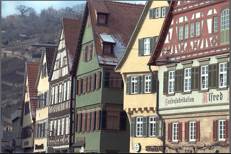
\includegraphics[width=1\textwidth]{24images/resize_kodim08.png}
\end{minipage}
\begin{minipage}{0.075\textwidth}
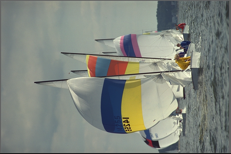
\includegraphics[width=1\textwidth]{24images/resize_kodim09.png}
\end{minipage}
\begin{minipage}{0.075\textwidth}
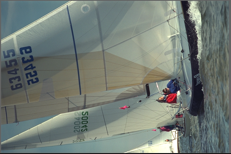
\includegraphics[width=1\textwidth]{24images/resize_kodim10.png}
\end{minipage}
\begin{minipage}{0.075\textwidth}
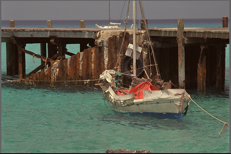
\includegraphics[width=1\textwidth]{24images/resize_kodim11.png}
\end{minipage}
\begin{minipage}{0.075\textwidth}
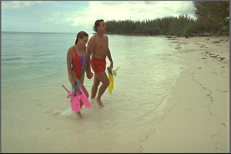
\includegraphics[width=1\textwidth]{24images/resize_kodim12.png}
\end{minipage}
}\vspace{-3mm}
\subfigure{
\begin{minipage}{0.075\textwidth}
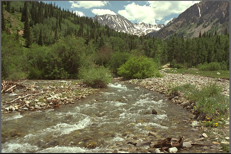
\includegraphics[width=1\textwidth]{24images/resize_kodim13.png}
\end{minipage}
\begin{minipage}{0.075\textwidth}
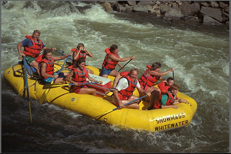
\includegraphics[width=1\textwidth]{24images/resize_kodim14.png}
\end{minipage}
\begin{minipage}{0.075\textwidth}
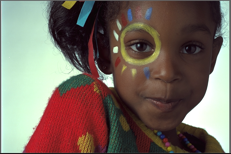
\includegraphics[width=1\textwidth]{24images/resize_kodim15.png}
\end{minipage}
\begin{minipage}{0.075\textwidth}
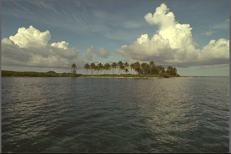
\includegraphics[width=1\textwidth]{24images/resize_kodim16.png}
\end{minipage}
\begin{minipage}{0.075\textwidth}
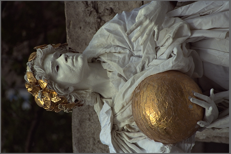
\includegraphics[width=1\textwidth]{24images/resize_kodim17.png}
\end{minipage}
\begin{minipage}{0.075\textwidth}
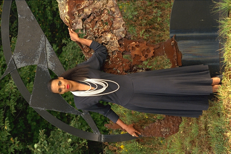
\includegraphics[width=1\textwidth]{24images/resize_kodim18.png}
\end{minipage}
}\vspace{-3mm}
\subfigure{
\begin{minipage}{0.075\textwidth}
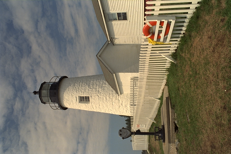
\includegraphics[width=1\textwidth]{24images/resize_kodim19.png}
\end{minipage}
\begin{minipage}{0.075\textwidth}
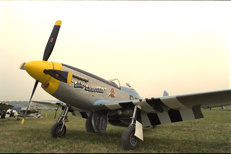
\includegraphics[width=1\textwidth]{24images/resize_kodim20.png}
\end{minipage}
\begin{minipage}{0.075\textwidth}
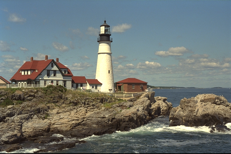
\includegraphics[width=1\textwidth]{24images/resize_kodim21.png}
\end{minipage}
\begin{minipage}{0.075\textwidth}
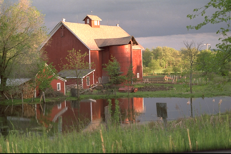
\includegraphics[width=1\textwidth]{24images/resize_kodim22.png}
\end{minipage}
\begin{minipage}{0.075\textwidth}
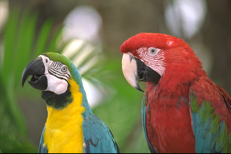
\includegraphics[width=1\textwidth]{24images/resize_kodim23.png}
\end{minipage}
\begin{minipage}{0.075\textwidth}
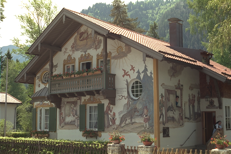
\includegraphics[width=1\textwidth]{24images/resize_kodim24.png}
\end{minipage}
}\vspace{1mm}
\caption{The 24 high quality color images from the Kodak PhotoCD Dataset.}
\label{f2}
\vspace{-2mm}
\end{figure}


\begin{table*}
\caption{PSNR(dB) results of different denoising algorithms on 24 natural images.}
\label{taba}
\begin{center}
\renewcommand\arraystretch{1.0}
\scriptsize
\begin{tabular}{|c||c|c|c|c|c|c|c|c|c|}
\hline
&\multicolumn{9}{c|}{ $\sigma_{r} = 40, \sigma_{g} = 20, \sigma_{b} = 30$}
\\
\hline
\hline
Image\#
&
\textbf{CBM3D}
&
\textbf{MLP}
&
\textbf{TNRD}
&
\textbf{NI}
&
\textbf{NC}
&
\textbf{WNNM0}
&
\textbf{WNNM1}
&
\textbf{WNNM2}
&
\textbf{MC-WNNM}
\\
\hline
1& 25.24 & 25.70 & 25.74 & 23.85 & 24.90 & 26.01 & 25.95 & 25.58 & \textbf{26.66}
\\
\hline
2& 28.27 & 30.12 & 30.21 & 25.90 & 25.87 & 30.08 & 30.11 & 29.80 & \textbf{30.20} 
\\
\hline
3 & 28.81 & 31.19 & 31.49 & 26.00 & 28.58 & 31.58 & 31.61 & 31.20 & \textbf{32.25}  
\\
\hline 
4 & 27.95 & 29.88 & 29.86 & 25.82 & 25.67 & 30.13 & 30.16 & 29.84 & \textbf{30.49} 
\\
\hline
5 & 25.03 & 26.00 & 26.18 & 24.38 & 25.15 & 26.44 & 26.39 & 25.32 & \textbf{26.82}
\\
\hline
6 & 26.24 & 26.84 & 26.90 & 24.65 & 24.74 & 27.39 & 27.30 & 26.88 & \textbf{27.98} 
\\
\hline
7 & 27.88 & 30.28 & 30.40 & 25.63 & 27.69 & 30.47 & 30.54 & 29.70 & \textbf{30.98} 
\\
\hline
8 & 25.05 & 25.59 & 25.83 & 24.02 & 25.30 & 26.71 & 26.75 & 25.26 & \textbf{26.90}
\\
\hline
9 & 28.44 & 30.75 & 30.81 & 25.94 & 27.44 & 30.86 & 30.92 & 30.29 & \textbf{31.49}
\\
\hline
10 & 28.27 & 30.38 & 30.57 & 25.87 & 28.42 & 30.65 & 30.68 & 29.95 & \textbf{31.26}
\\
\hline
11 & 26.95 & 28.00 & 28.14 & 25.32 & 24.67 & 28.19 & 28.16 & 27.61 & \textbf{28.63}
\\
\hline
12 & 28.76 & 30.87 & 31.05 & 26.01 & 28.37 & 30.97 & 31.06 & 30.58 & \textbf{31.48}
\\
\hline
13 & 23.76 & 23.95 & 23.99 & 23.53 & 22.76 & 24.27 & 24.15 & 23.52 & \textbf{24.89}
\\
\hline
14 & 26.02 & 26.97 & 27.11 & 24.94  & 25.68 & 27.20 & 27.15 & 26.55 & \textbf{27.57}
\\
\hline
15 & 28.38 & 30.15 & 30.44 & 26.06 & 28.21 & 30.52 & 30.60 & 30.13 & \textbf{30.81}
\\
\hline
16 & 27.75 & 28.82 & 28.87 & 25.69 & 26.66 & 29.27 & 29.21 & 29.02 & \textbf{29.96}
\\
\hline
17 & 27.90 & 29.57 & 29.80 & 25.85 & 28.32 & 29.78 & 29.79 & 29.16 & \textbf{30.40}
\\
\hline
18 & 25.77 & 26.40 & 26.41 & 24.74 & 25.70 & 26.63 & 26.56 & 26.01 & \textbf{27.22}
\\
\hline
19 & 27.30 & 28.67 & 28.81 & 25.40 & 26.52 & 29.19 & 29.22 & 28.67 & \textbf{29.57}
\\
\hline
20 & 28.96 & 30.40 & 30.76 & 24.95 & 25.90 & 30.79 & 30.83 & 29.97 & \textbf{31.07}
\\
\hline
21 & 26.54 & 27.53 & 27.60 & 25.06 & 26.48 & 27.80 & 27.75 & 27.12 & \textbf{28.34}
\\
\hline
22 & 27.05 & 28.17 & 28.27 & 25.36 & 26.60 & 28.21 & 28.16 & 27.81 & \textbf{28.64}
\\
\hline
23 & 29.14 & 32.31 & 32.51 & 26.13 & 23.24 & 31.89 & 31.97 & 31.21 & \textbf{32.34}
\\
\hline
24 & 25.75 & 26.41 & 26.53 & 24.55 & 25.73 & 27.10 & 27.03 & 26.18 & \textbf{27.59}
\\
\hline
\textbf{Average} & 27.13 & 28.54 & 28.68 & 25.24 & 26.19 & 28.84 & 28.83 & 28.22 & \textbf{29.31}
\\
\hline
\end{tabular}
\end{center}
\vspace{-3mm}
\end{table*}

\begin{figure*}\vspace{1mm}
\centering
\subfigure{
\begin{minipage}[t]{0.195\textwidth}
\centering
\raisebox{-0.15cm}{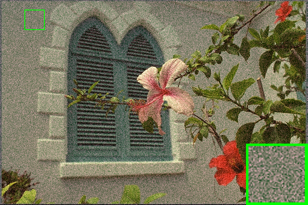
\includegraphics[width=1\textwidth]{comparea/resize_br_Noisy_nSig402030_kodim07.png}}
{\footnotesize (a) Noisy kodim07: 37.00dB }
\end{minipage}
\begin{minipage}[t]{0.195\textwidth}
\centering
\raisebox{-0.15cm}{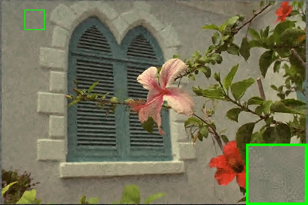
\includegraphics[width=1\textwidth]{comparea/resize_br_CBM3D_nSig402030_kodim07.png}}
{\footnotesize (b) CBM3D \cite{cbm3d}: 37.02dB}
\end{minipage}
\begin{minipage}[t]{0.195\textwidth}
\centering
\raisebox{-0.15cm}{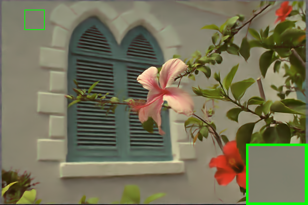
\includegraphics[width=1\textwidth]{comparea/resize_br_MLP_nSig402030_kodim07.png}}
{\footnotesize (c) MLP \cite{mlp}: 37.01dB}
\end{minipage}
\begin{minipage}[t]{0.195\textwidth}
\centering
\raisebox{-0.15cm}{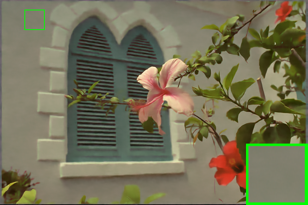
\includegraphics[width=1\textwidth]{comparea/resize_br_TNRD_nSig402030_kodim07.png}}
{\footnotesize (d) TNRD \cite{chen2015learning}: 33.90dB }
\end{minipage}
\centering
\begin{minipage}[t]{0.195\textwidth}
\raisebox{-0.15cm}{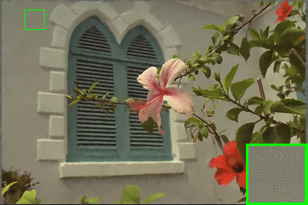
\includegraphics[width=1\textwidth]{comparea/resize_br_NC_nSig402030_kodim07.png}}
{\footnotesize (e) NC \cite{noiseclinic,ncwebsite}: 36.18dB  } 
\end{minipage}
}\vspace{-3mm}
\subfigure{
\begin{minipage}[t]{0.195\textwidth}
\centering
\raisebox{-0.15cm}{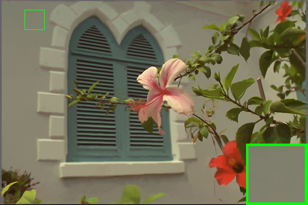
\includegraphics[width=1\textwidth]{comparea/resize_br_WNNMCW_nSig402030_kodim07.png}}
{\footnotesize (f) WNNM0: 37.68dB  }
\end{minipage}
\begin{minipage}[t]{0.195\textwidth}
\centering
\raisebox{-0.15cm}{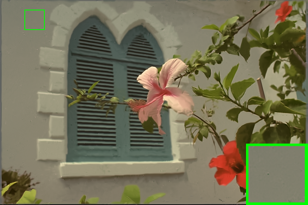
\includegraphics[width=1\textwidth]{comparea/resize_br_WNNMJ_nSig402030_kodim07.png}}
{\footnotesize (g) WNNM1: 38.76dB  }
\end{minipage}
\begin{minipage}[t]{0.195\textwidth}
\centering
\raisebox{-0.15cm}{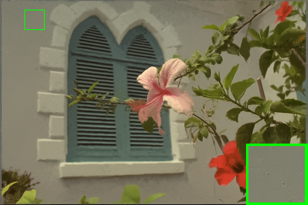
\includegraphics[width=1\textwidth]{comparea/resize_br_WNNM_ADMM_nSig402030_kodim07.png}}
{\footnotesize (h) WNNM2: 38.37dB }
\end{minipage}
\begin{minipage}[t]{0.195\textwidth}
\centering
\raisebox{-0.15cm}{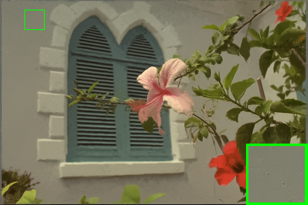
\includegraphics[width=1\textwidth]{comparea/resize_br_WNNM_ADMM_nSig402030_kodim07.png}}
{\footnotesize (i) MC-WNNM: \textbf{40.50}dB}
\end{minipage}
\begin{minipage}[t]{0.195\textwidth}
\centering
\raisebox{-0.15cm}{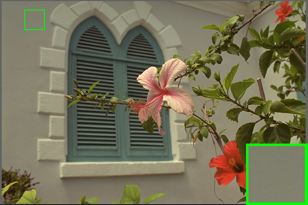
\includegraphics[width=1\textwidth]{comparea/resize_br_kodim07.png}}
{\footnotesize (j) kodim07}
\end{minipage}
}\vspace{-0.5mm}
\caption{Denoised images of different methods on the image ``kodim07'' degraded by noise with different levels on different channels. The images are better to be zoomed in on screen.}
\label{f3}
\vspace{-3mm}
\end{figure*}

\begin{figure}
\centering
\subfigure{
\begin{minipage}{0.085\textwidth}
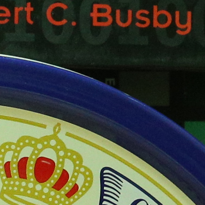
\includegraphics[width=1\textwidth]{CC15images/resize_5dmark3_iso3200_1_real.png}
\end{minipage}
\begin{minipage}{0.085\textwidth}
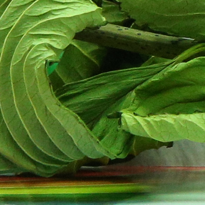
\includegraphics[width=1\textwidth]{CC15images/resize_5dmark3_iso3200_2_real.png}
\end{minipage}
\begin{minipage}{0.085\textwidth}
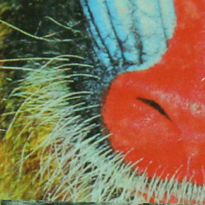
\includegraphics[width=1\textwidth]{CC15images/resize_5dmark3_iso3200_3_real.png}
\end{minipage}
\begin{minipage}{0.085\textwidth}
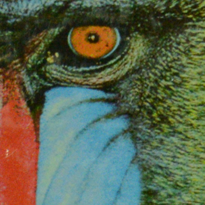
\includegraphics[width=1\textwidth]{CC15images/resize_d600_iso3200_1_real.png}
\end{minipage}
\begin{minipage}{0.085\textwidth}
\includegraphics[width=1\textwidth]{CC15images/resize_d600_iso3200_2_real.png}
\end{minipage}
}\vspace{-3mm}
\subfigure{
\begin{minipage}{0.085\textwidth}
\includegraphics[width=1\textwidth]{CC15images/resize_d600_iso3200_3_real.png}
\end{minipage}
\begin{minipage}{0.085\textwidth}
\includegraphics[width=1\textwidth]{CC15images/resize_d800_iso1600_1_real.png}
\end{minipage}
\begin{minipage}{0.085\textwidth}
\includegraphics[width=1\textwidth]{CC15images/resize_d800_iso1600_2_real.png}
\end{minipage}
\begin{minipage}{0.085\textwidth}
\includegraphics[width=1\textwidth]{CC15images/resize_d800_iso1600_3_real.png}
\end{minipage}
\begin{minipage}{0.085\textwidth}
\includegraphics[width=1\textwidth]{CC15images/resize_d800_iso3200_1_real.png}
\end{minipage}
}\vspace{-3mm}
\subfigure{
\begin{minipage}{0.085\textwidth}
\includegraphics[width=1\textwidth]{CC15images/resize_d800_iso3200_2_real.png}
\end{minipage}
\begin{minipage}{0.085\textwidth}
\includegraphics[width=1\textwidth]{CC15images/resize_d800_iso3200_3_real.png}
\end{minipage}
\begin{minipage}{0.085\textwidth}
\includegraphics[width=1\textwidth]{CC15images/resize_d800_iso6400_1_real.png}
\end{minipage}
\begin{minipage}{0.085\textwidth}
\includegraphics[width=1\textwidth]{CC15images/resize_d800_iso6400_2_real.png}
\end{minipage}
\begin{minipage}{0.085\textwidth}
\includegraphics[width=1\textwidth]{CC15images/resize_d800_iso6400_3_real.png}
\end{minipage}
}\vspace{-1mm}
\caption{The 15 cropped real noisy images used in \cite{crosschannel2016}.}
\label{f4}
\vspace{-3mm}
\end{figure}

\subsection{Experiments on Real Noisy Images}

In this section, we compare the proposed MC-WNNM method with other competing methods on the 15 real noisy images (Fig.\ \ref{f4}). We do not compare with the ``WNNM0'' method due to limited space and its inferior performance. The noisy images were collected under controlled indoor environment.\ Each scene was shot 500 times under the same camera and camera setting.\ The mean image of the 500 shots is roughly taken as the ``ground truth", with which the PSNR can be computed. Since the image size is very large (about $7000\times5000$) and the 11 scenes share repetitive contents, the authors of \cite{crosschannel2016} cropped 15 smaller images (of size $512\times512$) to perform experiments. For each real noisy image, the noise levels in R, G, B channels are estimated by \cite{Chen2015ICCV}. Since the noise levels are small in real noisy images, for the method of MLP \cite{mlp} and TNRD \cite{chen2015learning}, we apply the trained models of corresponding methods and choose the best denoising results (highest average PSNR values). Both methods achieves best results when setting the noise levels of the trained models from $\sigma=10$.  

We perform quantitative comparison on the 15 cropped images used in \cite{crosschannel2016}. The PSNR results are listed in Table \ref{tabb} of the compared methods including CBM3D \cite{cbm3d}, MLP \cite{mlp}, TNRD \cite{chen2015learning}, NC \cite{noiseclinic,ncwebsite}, NI \cite{neatimage},
CC \cite{crosschannel2016} (copied from \cite{crosschannel2016}), ``WNNM1'', ``WNNM2'', and the proposed MC-WNNM method.\ The highest PSNR results are highlighted in bold.\ On average PSNR, the proposed MC-WNNM method achieves 0.44dB improvements over the ``WNNM1'' method and outperforms the state-of-the-art denoising method CC \cite{crosschannel2016} by 0.83dB. On 10 out of the whole 15 images, the proposed MC-WNNM method achieves the highest PSNR values.\ Both CC and ``WNNM1'' achieves highest PSNR results on 2 of 15 images.\ It should be noted that in the CC method, a specific model is trained for each camera and camera setting, while our method uses the same model for all images.\ Fig.\ \ref{f5} shows the denoised images of a scene captured by Canon 5D Mark 3 at ISO = 3200.\ We can see that CBM3D, NC, NI and CC would either remain noise or generate artifacts, while TNRD over-smooth much the image.\ By using the proposed MC-WNNM model achieves better visual quality results than other methods.\ More visual comparisons can be found in the supplementary files.


\begin{table*}\vspace{2mm}
\caption{PSNR(dB) results of different methods on 15 cropped real noisy images used in \cite{crosschannel2016}.}
\vspace{0.5mm}
\label{tabb}
\begin{center}
\renewcommand\arraystretch{1}
\begin{tabular}{|c||c|c|c|c|c|c|c|c|c|}
\hline
Camera Settings  
&
\textbf{CBM3D}
&
\textbf{MLP}
&
\textbf{TNRD}
&
\textbf{NI}
&
\textbf{NC}
&
\textbf{CC}
&
\textbf{WNNM1}
&
\textbf{WNNM2}
&
\textbf{MC-WNNM} 
\\
\hline
\multirow{3}{*}{\small{Canon 5D Mark III}}  
& 39.76 & 39.00 & 39.51 & 35.68 & 36.20 & 38.37 & 39.74 & 39.98 & \textbf{41.13}
\\ 
\cdashline{2-10} 
\multirow{3}{*}{ISO = 3200}   
 & 36.40 & 36.34 & 36.47 & 34.03 & 34.35 & 35.37 & 35.12 & 36.65 & \textbf{37.28}
\\ 
\cdashline{2-10}    
 & 36.37 & 36.33 & 36.45 & 32.63 & 33.10& 34.91 & 33.14 & 34.63 & \textbf{36.52}  
\\
\hline
\multirow{3}{*}{Nikon D600} 
 & 34.18 & 34.70 & 34.79 & 31.78 & 32.28 & 34.98 & 35.08 & 35.08 & \textbf{35.53}
\\ 
\cdashline{2-10} 
\multirow{3}{*}{ISO = 3200}   
 & 35.07 & 36.20 & 36.37 & 35.16 & 35.34 & 35.95 & 36.42 & 36.84 & \textbf{37.02}
\\ 
\cdashline{2-10}    
 & 37.13 & 39.33 & 39.49 & 39.98 & 40.51 & \textbf{41.15} & 40.78 & 39.24 & 39.56
\\
\hline
\multirow{3}{*}{Nikon D800} 
 & 36.81  & 37.95 & 38.11 & 34.84 & 35.09 & 37.99 & 38.28 & 38.61 & \textbf{39.26}
\\ 
\cdashline{2-10} 
\multirow{3}{*}{ISO = 1600}   
 & 37.76 & 40.23 & 40.52 & 38.42 & 38.65 & 40.36 & 41.24 & 40.81 & \textbf{41.43}
\\ 
\cdashline{2-10}    
 & 37.51 & 37.94 & 38.17 & 35.79 & 35.85 & 38.30 & 38.04 & 38.96 & \textbf{39.55}
\\
\hline
\multirow{3}{*}{Nikon D800} 
 & 35.05 & 37.55 & 37.69 & 38.36 & 38.56 & \textbf{39.01} & 39.93 & 37.97 & 38.91
\\ 
\cdashline{2-10} 
\multirow{3}{*}{ISO = 3200}   
 & 34.07 & 35.91 & 35.90 & 35.53 & 35.76 & 36.75 & 37.32 & 37.30 & \textbf{37.41}
\\ 
\cdashline{2-10}    
 & 34.42 & 38.15 & 38.21 & 40.05 & 40.59 & 39.06 & \textbf{41.52} & 38.68 & 39.39
\\ 
\hline
\multirow{3}{*}{Nikon D800} 
& 31.13 & 32.69 & 32.81 & 34.08 & 34.25 & 34.61 & \textbf{35.20} & 34.57 & 34.80
\\ 
\cdashline{2-10} 
\multirow{3}{*}{ISO = 6400}   
 & 31.22 & 32.33 & 32.33 & 32.13 & 32.38  & 33.21 & 33.61 & 33.43 & \textbf{33.95}
\\ 
\cdashline{2-10}    
 & 30.97 & 32.29 & 32.29 & 31.52 & 31.76 & 33.22 & 33.62 & \textbf{34.02} & 33.94
\\
\hline
Average & 35.19 & 36.46 & 36.61 & 35.33 & 35.65 & 36.88 & 37.27 & 37.12 & \textbf{ 37.71}
\\
\hline
\end{tabular}
\end{center}
\vspace{1mm}
\end{table*}

\begin{figure*}\vspace{1mm}
\centering
\subfigure{
\begin{minipage}[t]{0.195\textwidth}
\centering
\raisebox{-0.15cm}{\includegraphics[width=1\textwidth]{compareb/resize_br_Noisy_5dmark3_iso3200_1.png}}
{\footnotesize (a) Noisy kodim07: 37.00dB }
\end{minipage}
\begin{minipage}[t]{0.195\textwidth}
\centering
\raisebox{-0.15cm}{\includegraphics[width=1\textwidth]{compareb/resize_br_CBM3D_CC15_5dmark3_iso3200_1.png}}
{\footnotesize (b) CBM3D \cite{cbm3d}: 39.76dB}
\end{minipage}
\begin{minipage}[t]{0.195\textwidth}
\centering
\raisebox{-0.15cm}{\includegraphics[width=1\textwidth]{compareb/resize_br_TRD_CC15_5dmark3_iso3200_1.png}}
{\footnotesize (c)  TNRD \cite{chen2015learning}: 39.51dB}
\end{minipage}
\begin{minipage}[t]{0.195\textwidth}
\centering
\raisebox{-0.15cm}{\includegraphics[width=1\textwidth]{compareb/resize_br_NI_CC15_5dmark3_iso3200_1.png}}
{\footnotesize (d) NI \cite{neatimage}: 35.68dB }
\end{minipage}
\centering
\begin{minipage}[t]{0.195\textwidth}
\raisebox{-0.15cm}{\includegraphics[width=1\textwidth]{compareb/resize_br_NC_CC15_5dmark3_iso3200_1.png}}
{\footnotesize (e) NC \cite{noiseclinic,ncwebsite}: 36.20dB  } 
\end{minipage}
}\vspace{-3mm}
\subfigure{
\begin{minipage}[t]{0.195\textwidth}
\centering
\raisebox{-0.15cm}{\includegraphics[width=1\textwidth]{compareb/resize_br_CC_CC15_5dmark3_iso3200_1.png}}
{\footnotesize (f) CC \cite{crosschannel2016}: 38.37dB  }
\end{minipage}
\begin{minipage}[t]{0.195\textwidth}
\centering
\raisebox{-0.15cm}{\includegraphics[width=1\textwidth]{compareb/resize_br_WNNMJ_CC15_5dmark3_iso3200_1.png}}
{\footnotesize (g) WNNM1: 39.74dB  }
\end{minipage}
\begin{minipage}[t]{0.195\textwidth}
\centering
\raisebox{-0.15cm}{\includegraphics[width=1\textwidth]{compareb/resize_br_WNNM_ADMM_NL_CC15_5dmark3_iso3200_1.png}}
{\footnotesize (h) WNNM2: 39.98dB }
\end{minipage}
\begin{minipage}[t]{0.195\textwidth}
\centering
\raisebox{-0.15cm}{\includegraphics[width=1\textwidth]{compareb/resize_br_CWNNM_ADMM_NL_CC15_5dmark3_iso3200_1.png}}
{\footnotesize (i) MC-WNNM: \textbf{41.13}dB}
\end{minipage}
\begin{minipage}[t]{0.195\textwidth}
\centering
\raisebox{-0.15cm}{\includegraphics[width=1\textwidth]{compareb/resize_br_5dmark3_iso3200_1.png}}
{\footnotesize (j) Mean Image}
\end{minipage}
}\vspace{-0.5mm}
\caption{Denoised images of a region cropped from the real noisy image ``Canon 5D Mark 3 ISO 3200 1" \cite{crosschannel2016} by different methods. The images are better to be zoomed in on screen.}
\label{f5}
\vspace{0.5mm}
\end{figure*}

\section{Conclusion and Future Work}

The real noisy images have different noise structures among the R, G, B channels due to the preprocessing steps of the digital camera pipelines in CCD or CMOS sensors. This makes the real image denoising problem much more complex than grayscale image denoising. In this paper, we proposed a noval multi-channel (MC) model for real color image denoising. By introducing a weighting matrix to the concatenated weighted nuclear norm minimization (WNNM) model, the proposed MC-WNNM model can process adaptively the different noise structures in each of the R, G, B channels and exploit the non-local self similarity property of natural images. Though no longer having closed-form solution, we successfully solved the MC-WNNM model via an ADMM algorithm by reformulating the MC-WNNM model as a linear equality-constrained problem with two separable variables. We also studied the convergence property of the ADMM algorithm. Extensive experiments on synthetic and real color image denoising demonstrate that, the proposed MC-WNNM model outperforms the other competing denoising methods on both synthetic color noisy images as well as real-world noisy images. The introduce of the weighting matrix can boost the performance of traditional models on new applications. We believe that this work can be extended in at least two directions. Firstly, the weighting matrix beyond the diagonal form, such as correlation form \cite{nearcor}, may bring better performance on color image denoising. Secondly, the proposed MC-WNNM model can be further extended to deal with hyperspectral images, which contain much more channels than color images.



{
\small
\bibliographystyle{unsrt}
\bibliography{egbib}
}

\end{document}